구간법은 함수가 근의 근처에서 부호(sign)가 변한다는 사실에 기초한다. 이 방법을 사용하여 근을 구하기 위해서는 두 개의 초기 가정값이 필요하기 때문에 구간법(bracketing method)이라고 부른다.

\subsection{도식적 방법}
방정식 $f(x)=0$에 대한 근사값을 구하기 위한 간단한 방법은 함수를 그려서 $x$축과 만나는 곳을 찾아보는 것이다. $f(x)=0$이 되게 하는 $x$값을 근의 대락적인 근사값으로 간주할 수 있다.
\\
\framebox{예제} \textbf{도식적 방법}\\
\rule{\textwidth}{0.1pt}
도식적 방법을 사용하여 질량 $m=68.1$kg인 낙하산병이 자유 낙하 10초 후에 $40m/s$의 속도를 갖도록 하는 제동계수를 구하라(단, 중력에 의한 가속도는 $9.8m/s^2$이다).
\\
\framebox{해}
식(\ref{eq:1-11})에서 제동계수인 $c$를 내재적(implicit) 매개변수로 포함시키면
\begin{equation}
f(c)=\frac{gm}{c}\left(1-e^{-(c/m)t}\right)-v
\end{equation}
과 같이 쓸 수 있다. 즉, 매개변수 $t=10$,$g=9.8$,$v=40$,$m=68.1$ 이 주어진 $c$에 대한 함수$f(c)$로 쓸 수 있다.
\begin{equation}
f(c)=\frac{9.8\times68.1}{c}\left(1-e^{-(c/68.1)\times10}\right)-40
\label{eq:e5-1-1}
\end{equation}

다양한 $c$의 값을 대입하여 $f(c)$값을 계산한다. (MATLAB 활용)
\lstinputlisting[language=Matlab, label=lst:mylist,caption= 도식적 방법으로 방정식의 근 구하기]{MATLAB/brack1.m} 
\begin{figure}[!hbpt]
\centering
\includegraphics[keepaspectratio=true,width=0.8\linewidth]{figs/5-1.eps}
\caption{방정식의 근을 구하기 위하여 도식적(그래프를 사용하는) 방법}
\label{fig:5-1}
\end{figure}

\clearpage
\subsection{이분법}
일반적으로 $f(x)$가 구간 $x_l$과 $x_u$사이에서 실수이고 연속이며, $f(x_{l})$과 $f(x_{u})$가 반대 부호를 갖는다면, 즉
\begin{equation}
f(x_{l})(x_{u})<0
\end{equation}
이면 $x_{l}$과 $x_{u}$사이에는 적어도 하나 이상의 실근(real root)이 존재한다.
\begin{itemize}
\item 증분탐색법(incremental search method) : 함수의 부호가 변화하는 구간을 찾아내어 근을 구하는 방법. 부호가 변하는 위치는 구간을 보다 작은 소구간으로 나눔으로써 정밀하게 식별할 수 있다.
\item 이분법(bisection method) : 이진 버림(binary chopping), 구간 반분법(interval halving) 또는 Bolzano법이라고도 부른다. 이분법은 증분탐색법의 하나로 구간을 항상 반으로 나눈다. 만일 함수의 부호가 구간내에서 바뀐다면 구간의 중간점에서 함수값을 계산한다.
\end{itemize}
%\begin{tabular}[c]{|p{\textwidth}|}
\begin{tabular}[t]{|i{0.001cm}e{0.9\textwidth}|}
\hline
  \item[]
  \item[]
  \item[]&
  \item[\textbf{Step 1}] Choose lower $x_{l}$ and upper $x_{u}$ guesses for the root such that the function changes sign over the interval. This can be checked by ensuring that $f(x_{l})f(x_{u})<0$.
  \item[\textbf{Step 2}]  An estimate of the root $x_{r}$ is determined by
\begin{displaymath}
x_{r}=\frac{x_{l}+x_{u}}{2}
\end{displaymath}
  \item[\textbf{Step 3}] Make the following evaluations to determine in which subinterval the root lies:
  \begin{itemize}
  \item[(a)] if $f(x_{l})f(x_{r})<0$, the root lies in the lower subinterval. Therefore, set $x_{u}=x_{r}$ and return to \textbf{Step 2}.
  \item[(b)] if $f(x_{l})f(x_{r})>0$, the root lies in the upper subinterval. Therefore, set $x_{l}=x_{r}$ and return to \textbf{Step 2}.
  \item[(c)] if $f(x_{l})f(x_{r})=0$, the root equals $x_{r}$; terminate the computation.
  \end{itemize}
\\\hline
\end{tabular}

도식적 방법의 예제에서 식(\ref{eq:e5-1-1})를 이분법을 이용해서 풀어보자.
\\
\framebox{예제} \textbf{이분법}\\
\rule{\textwidth}{0.1pt}

\lstinputlisting[language=Matlab, label=lst:5-2,caption=식(\ref{eq:e5-1-1})의 함수 정의]{MATLAB/f.m}
Code~\ref{lst:5-2}와 같이 식(\ref{eq:e5-1-1})을 함수화 시키자. 그리고 이분법 연산은
\lstinputlisting[language=Matlab, label=lst:5-3,caption=식(\ref{eq:e5-1-1})의 이분법 코드]{MATLAB/bisec1.m}
Code~\ref{lst:5-3}과 같이 반복문(loop)와 조건문(selection)으로 이뤄진다. 여기서는 \texttt{while}문을 사용하여 코딩을 하였는데, 이것은 반복문의 반복횟수로 종료판정을 하지 못하기 때문이다. \texttt{while}문은 \texttt{while} 이후에 조건을 입력해야 하지만 여기서는 여러조건이 함께 존재하기 때문에 \texttt{1} 즉, 무한반복을 선택하였다. 대신 \texttt{if}문과 \texttt{elseif} 그리고 \texttt{else} 문을 사용하였고 종료판정은 \texttt{else}에 \texttt{break}를 사용하여 반복을 종료하게 된다.

\subsubsection{종료 판정 기준과 오차추정}
실제로 예제의 정확한 값을 얻기 위해서 이분법을 반복시킬 수 있지만, 실제로 컴퓨터 연산은 일반적인 경우 $f(x_{r})=0$이 되는 경우까지 하는것은 매우 비효율 적이고, 복잡한 수치모델의 경우 반복문이 끝나지 않을 수가 있다. 따라서 언제 이 반복문을 끝낼 것인지에 대한 객관적인 판정 기준을 제시해야한다.\\
예를들어 오차가 미리 정한 정밀도 이하로 떨어지면 계산을 종료한다고 생각해보자. 상대오차가 0.1\% 이하로 떨어지면 계산을 종료한다고 가정하면 문제가 발생한다. 왜냐하면 우리는 참값을 알지 못하기 때문에 상대오차를 계산할 수 없디 때문이다. 참값을 안다면 굳이 이분법 같은 수치해법으로 근을 구할 필요가 없기 때문이다. 하지만 \pageref{sec:3-2}페이지 \ref{sec:3-2}절에서 식(\ref{eq:3-5})를 통해 근사화된 상대오차를 구한적이 있다. 즉, 식(\ref{eq:5-2})와 같이 반복계산문에서 이전의 값과 현재의 값의 변화로 판별하여 근사상대오차를 구한다.
\begin{equation}\label{eq:5-2}
e_{a}=\left|\frac{x_{r}^{new}-x_{r}^{old}}{x_{r}^{new}}\right|100(\%)
\end{equation}

\subsubsection{함수 계산의 최소화}
Code~\ref{lst:5-3}과 같은 알고리즘은 계산하기 쉬운 함수의 단일근을 찾는 경우에는 유용하게 사용될 수 있으나 실제 공학 문제에서 이와 같은 경우는 드물다. 예를들어 많은 근을 찾아야하는 프로그램을 개발하는 경우, Code~\ref{lst:5-2}와 같은 알고리즘을 수천, 수백만번 수행할 수 도 있다. 또한 함수의 경우 간단하게 처리하는(수행시간이 짧은) 함수가 아닌 경우가 더 많다. 특히 연산 시간이 많이 소요되는 경우 우리는 함수계산을 최소화 시켜야 한다. 
변경된 코드를 보자
\lstinputlisting[language=Matlab, label=lst:5-4,caption=함수계산을 최소화한 이분법 코드]{MATLAB/bisec2.m}
즉 Code~\ref{lst:5-3}에서 $2n$번 수행이 되는 함수연산을 Code~\ref{lst:5-4}에서 $n+1$으로 축소시켰다. (여기서 $n$은 반복문의 반복횟수 \texttt{ii})

\subsection{가위치법}
이분법이 단일근을 찾는데에는 우수한 기법이지만 근에 접근하는 방식은 상당히 비효율적이다. 이분법의 단점은 구간 $x_{l}$과 $x_{u}$ 사이를 항상 반으로 나누고, 함수값 $f(x_{l})$과 $f(x_{u})$의 크기를 고려하지 않는다. 가위치법은 이러한 단점을 고려하여 $f(x_{l})$과 $f(x_{u})$ 사이의 곡선을 직선으로 연결시켜 $x$축과 만나는 교점을 찾아 그 교점이 추정값이 되는 방식이다. 곡선을 직선으로 대치하여 근의 \textsf{''가위치법''}(false position method), 또는 라틴어로 \textsf{''정규거짓''}(regula falsi)이라고 하며, \textsf{''선형보간법''}(linear interpolation method)라고도 한다.
\begin{equation}\label{eq:5-6}
\frac{f(x_{l})}{x_{r}-x_{l}}=\frac{f(x_{u})}{x_{r}-x_{u}}
\end{equation}
위의 식(\ref{eq:5-6})은 다음과 같이 정리할 수 있다.
\begin{equation}\label{eq:5-7}
x_{r}=x_{u}-\frac{f(x_{u})(x_l -x_u)}{f(x_l)-f(x_u)}
\end{equation}
\clearpage
즉, 식(\ref{eq:5-7})로 $x_{r}$의 값을 계산한 후, 두 개의 초기경계값 $x_{l}$ 또는 $x_{u}$ 중 하나로 대치하고, $f(x_{r})$과 같은 부호를 가진 함수값을 산출한다. 이 방법으로 $x_{l}$과 $x_{u}$의 사이에는 항상 참근이 존재하게 된다. 정확한 근을 구할 때 까지 이 과정을 반복한다. 이 알고리즘은 이분법의 \textbf{Step 2}에서 식(\ref{eq:5-7})을 사용하는 것을 제외하고 이분법과 같다.

\begin{figure}[!hbpt]
\centering
\includegraphics[keepaspectratio=true,width=0.6\linewidth]{figs/fpm1.eps}
\caption{가위치법의 도식적 묘사}
\label{fig:5-12}
\end{figure}

이분법과 같은 방식으로 낙하산병 예제를 풀어보자
\lstinputlisting[language=Matlab, label=lst:5-5,caption=식(\ref{eq:e5-1-1})의 가위치법 코드]{MATLAB/fpm1.m}
이분법과 가위치법의 상대적인 효율성을 비교해보자, 반복횟수에 대한 참상대오차가 줄어드는 경향을 판단해볼 수 있다.
\begin{figure}[!hbpt]
\centering
\subfigure[Short Iteration]{
\includegraphics[keepaspectratio=true,width=0.4\linewidth]{figs/compfnb1.eps}}
\subfigure[Full Iteration]{
\includegraphics[keepaspectratio=true,width=0.4\linewidth]{figs/compfnb2.eps}}
\caption{이분법과 가위치법 상대오차 비교}
\label{fig:5-12}
\end{figure}
\subsection{수정된 가위치법}
\begin{equation}\label{eq:e5-6}
f(x)=x^{10}-1
\end{equation}
식(\ref{eq:e5-6})의 경우 이분법이 가위치법보다 빠르게 수렴한다. 이것은 근을 찾는 방법을 일반화하는 것은 불가능하다는 것을 보여준다. 즉, 이것은 수정된 가위치법을 통해서 한쪽 경계가 변하지 않는 경우 알아내는 알고리즘을 포함시키는 것이다. 
\lstinputlisting[language=Matlab, label=lst:5-5,caption=식(\ref{eq:e5-6})의 수정된 가위치법 코드]{MATLAB/fpm22.m}
이러한 기존의 조건문에 또다른 조건문을 포함시켜 알고리즘을 추가하는 방식은 추후 증분탐색과 초기가정값의 크기에 따라 탐색을 놓칠 경우가 있기 때문에, 완전한 방법이라고 볼 수는 없다.

Figure~\ref{fig:5-13}을 통해 식(\ref{eq:e5-6})의 이분법, 가위치법, 수정된 가위치법의 참상대오차의 수렴과정을 살펴보자.
식(\ref{eq:e5-6}) 문제의 이분법, 가위치법의 각각의 MATLAB 코드는 \pageref{ap:3}페이지의 부록\ref{ap:3}장을 참고.\\
\clearpage
\begin{figure}[!hbpt]
\centering
\subfigure[Short Iteration]{
\includegraphics[keepaspectratio=true,width=0.4\linewidth]{figs/compfnbnm1.eps}}
\subfigure[Full Iteration]{
\includegraphics[keepaspectratio=true,width=0.4\linewidth]{figs/compfnbnm2.eps}}
\caption{이분법과 가위치법 및 수정된 가위치법 상대오차 비교}
\label{fig:5-13}
\end{figure}

Figure~\ref{fig:5-13-1}에서 이분법, 가위치법 그리고 수정된 가위치법이 단계별로 어떻게 근으로 수렴하는지 알 수 있다.

\begin{figure}[!hbpt]
\centering
\subfigure[Bisection method]{
\includegraphics[keepaspectratio=true,width=0.3\linewidth]{figs/bisecprocplot.eps}}
\subfigure[False position method]{
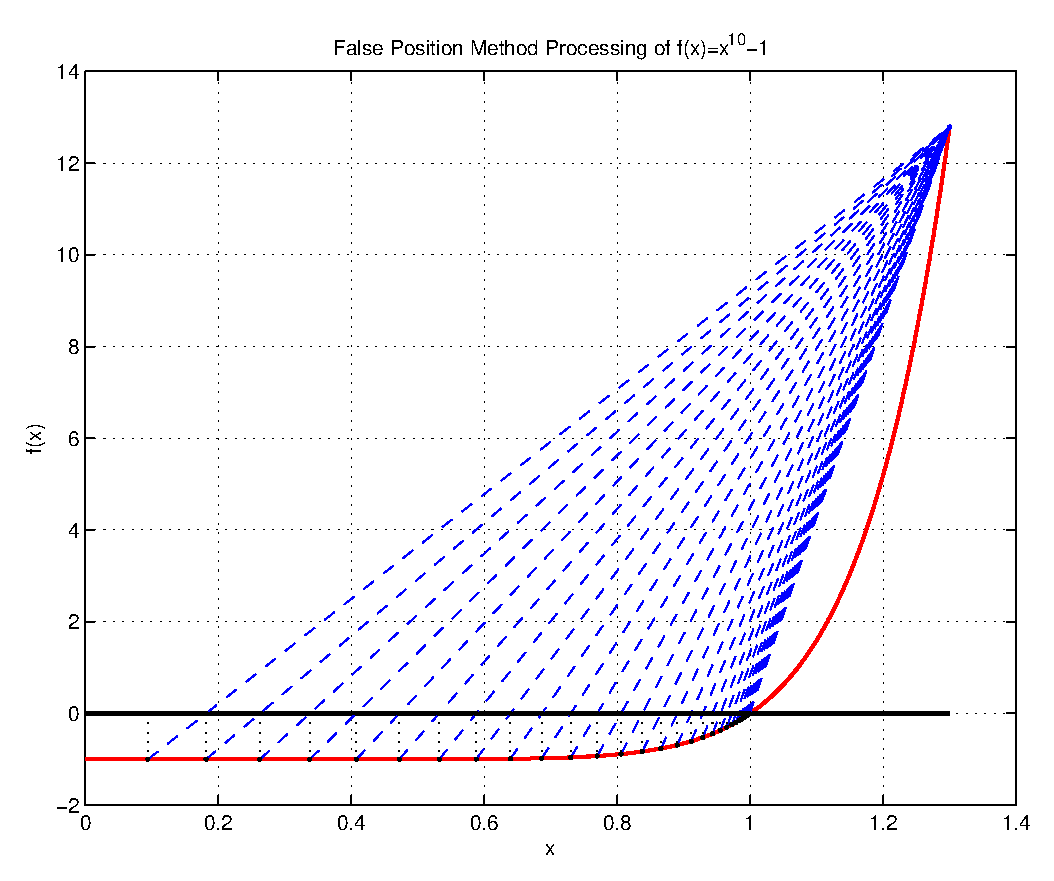
\includegraphics[keepaspectratio=true,width=0.3\linewidth]{figs/fpmprocplot.eps}}
\subfigure[Modified false position method]{
\includegraphics[keepaspectratio=true,width=0.3\linewidth]{figs/mfpmprocplot.eps}}
\caption{이분법과 가위치법 및 수정된 가위치법의 계산과정}
\label{fig:5-13-1}
\end{figure}

